
\section{Design}
\label{section:design}
\begin{figure*}
    \centering
    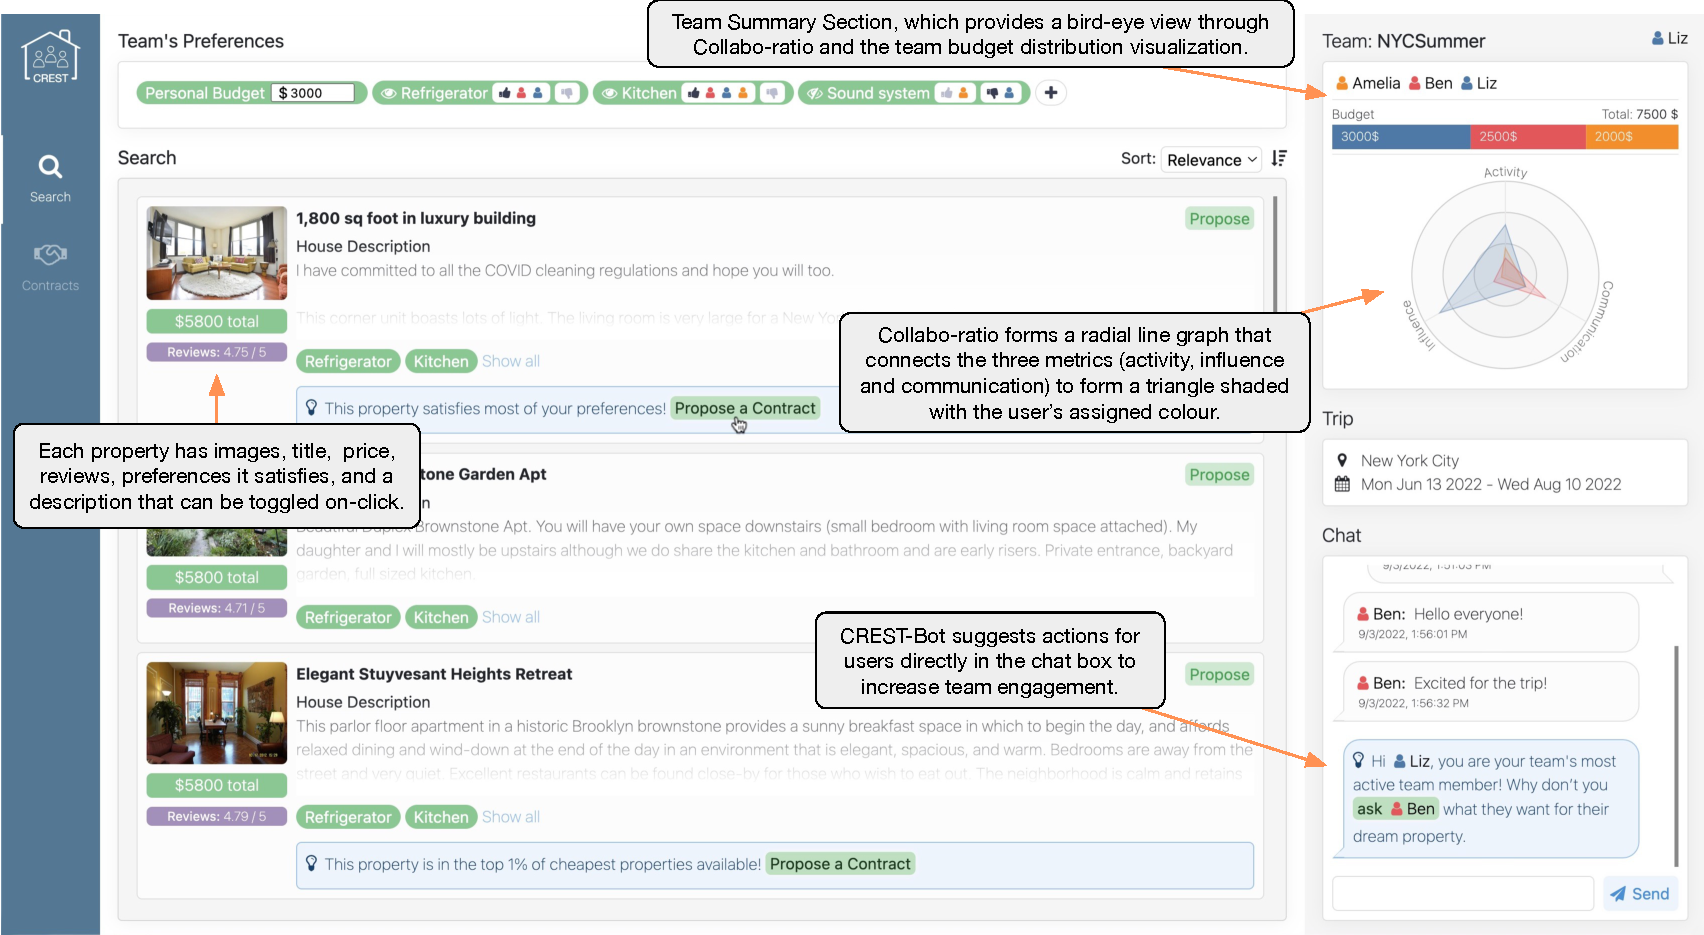
\includegraphics[width=\textwidth]{images/ui-search.pdf}
    \caption{A screenshot of \tool showing the search page, a visualization of the team's budget, a visualization of team engagement metrics, \collaboRatio, and the chat panel.}
    \label{fig:ui_search}
\end{figure*}

The motivation for \tool came from multiple conversations with individuals who struggle with property bookings. In particular, university students that need to find shared and affordable semester-long housing and family members looking for vacation rentals for family reunions. As we realized that current online-booking tools do not adequately support these users, we examined the literature to understand why. We found that collaborative search tools \cite{searchtogether, groupdynamicscollaborativesearch, c-dq,shareonewiki,resultsspace,slacksearch,algorithmiccollaborativesearch} address various crucial elements of collaborative search, but lack support for reaching agreement. Informed by the prior work, our design process defines the tasks, and outlines the challenges involved in group-rental-booking to put forward a set of design principles that shape \tool.


\subsection{Task Analysis}
\label{ssection:task}

We identify three broad group-rental-booking actions: \textit{search, discuss and agree}. In search, users explore the space of available properties. In discussion, users communicate with each other to share their search findings, their personal living requirements, constraints and property preferences. In agreement, users often work to convince each other of a few selected properties to finally settle on booking one. 
We break down these three main actions into the following five finer-grained tasks. While these tasks may seem sequential, we find that users often engage in them in no specific order, simultaneously and repeatedly.


\begin{enumerate}[label={}, leftmargin=0cm, itemindent=0.2cm]

\item \tIntrospection In this task (aka. private preparation \cite{pocketnegotiator}), users self-reflect to determine the properties of their ideal home. At several points throughout the group booking process, users might reevaluate their personal requirements leading to additional or different search criteria. Examining  the results of a search or discussing and understanding the preferences of the other group members can lead to further introspection where users better articulate their needs and wants. 

\item \tSearch  In this task, users specify their search criteria through the search engine's filters and sift through the results to find properties that satisfy either their individual criteria --- \textit{individual search} --- or at least a subset of the group's criteria in addition to their own --- \textit{joint search} \cite{resultsspace}. Users will often make a note of the properties they like through wishlists, bookmarks, etc. to revisit later for further ranking and eventually for selecting and sharing with the group their top properties.

\item \tInformationExchange  Users need to exchange information with each other regarding their preferences, budgets, search findings and top picks, and rules for co-living, which may include room allocation or assigned chores, to name a few. This information exchange can occur through different channels: chat messages, emails, verbal conversations, etc. Regardless of how information is exchanged among group members, it is crucial for the success of the overall group booking process \cite{meetingmediator}.
 
\item \tNegotiation  In many situations, group members may have different and diverging preferences. Yet, to successfully agree on a certain property, its supporting members might engage in different negotiation strategies to make it more appealing to the opposing members, such as  \textit{convincing} --- e.g. describing the merits of the proposed property or the drawbacks of alternative ones \cite{meetingmediator} --- 
    \textit{trading or bartering} --- e.g. agreeing to pay more or to provide transportation, to cook meals, etc. \cite{pocketnegotiator} --- 
    \textit{fair resource allocation} --- e.g. scheduling loud and quiet use periods for shared spaces, allocating rooms, bathrooms, or other amenities by needs \cite{fairresourceallocation}. 
    The opposing members can also engage in \textit{compromising} strategies where they agree to a less-desired property for the overall group's satisfaction or in return for a negotiated perk.

\item \tAgreement  In this task, users clearly signal their agreement to proceed with booking a specific property. It might take several rounds of confirmation or acknowledgement. Individual agreements can be broadcast to the entire group or through a leader that will complete the booking on behalf of the group members. It may also take several forms, from signing a formal contract that clearly lists the rental terms, each group member's financial contributions, space sharing and usage, and co-living rules to less formal methods such as verbally agreeing to a booking.

\end{enumerate}

\subsection {Challenges}
\label{ssection:challenges}


Several challenges hinder the success of asynchronous collaborative search and agreement for property booking, even among a group of friends. We now describe some of these challenges. Our design principles (Section \ref{ssection:principles}) aim to address these challenges.

\begin{enumerate}[label={}, leftmargin=0cm, itemindent=0.2cm]

    \item \cDisconnectedTooling As stated in Section \ref{ssection:task}, the tasks involved in collectively booking a property are roughly categorized into \textit{search, discuss and agree}. Yet, there are no tools that support \textit{all} three main task categories. Tools like SearchTogether \cite{searchtogether} provide features for collaborative search and discussion\footnote{\citeauthor{collaborativesearchrevisted} notes that users often repurpose external communication tools to satisfy their collaborative search needs beyond the search tools~\cite{collaborativesearchrevisted}.} but do not consider agreement, and tools like Spliddit \cite{spliddit} and PocketNegotiator \cite{pocketnegotiator} offer some mechanisms for agreement through bidding and algorithmically deciding fair contributions, but they do not consider search and have limited discussion features. Search and agreement, however, are very tightly connected in group booking: Failing to agree on a certain property may instantiate a new search where the group members are more cognizant of the factors that led to disagreement, and an awareness of the results from past independent or joint search efforts may help individuals better negotiate when trying to agree on booking a specific property. 

    
    \item \cDiscontinuity In large groups where members are potentially spread out over different time zones and the asynchronous collaborative work spans many days, individuals may have difficulty tracking the progress overall and feel that their individual efforts are discontinuous and disconnected from others. Consider Harish and Atul, who both live in Delhi and are planning their summer trip to Europe with Jawad, who lives in Vancouver. Harish and Atul have found and settled on two possible properties, but they failed to communicate their findings in time to Jawad; Jawad starts an independent search, not knowing what his friends have already found. When the friends later meet or exchange information, perhaps through email, Jawad may feel that his independent search efforts were wasted, an issue that \citeauthor{searchtogether} pointed out as a byproduct of a lack of awareness in collaborative search tools~\cite{searchtogether}. Moreover, if their property selections differ drastically, the ensuing conflict might be more difficult to resolve. From a tooling perspective, discontinuity can also be described as the lack of a centralized and persistent repository of each group member's preferences, constraints, favoured properties and agreement progress leading to the \textit{duplication of effort}~\cite{searchtogether} or a sense of discontinuity across the group's individual search and agreement efforts.
    
    \item \cShiftingGoalPosts Search tools, in general, aim to maximize \textit{recall}: finding all relevant records for given search criteria. In many collaborative search scenarios, high recall is the desired feature. For example, a group of researchers conducting a systematic review on a subject are interested in collating \textit{all} relevant research papers. A high-recall collaborative search task is inherently expansive. This contrasts with the goal of collaborative search in our setting, which is to find \textit{one} property that everyone agrees to. While generating a list of viable options for a group to examine and choose from is desirable, continuing the search even after the group members have largely settled on one or two options is counter-productive. More choices to consider can overwhelm some users, and individually exploring each one might be detrimental to the team's shared goal \cite{themediationprocess}. A group member may stall the agreement process by constantly expanding the search list (i.e. production-blocking by an over-participator \cite{meetingmediator}). Current search features such as bookmarks are better suited for list generation than property agreement: It is relatively easy for each group member to bookmark several properties without seriously considering their viability in terms of group fit. Thus, without a clear goal-oriented process that concludes the search, the sense of a \textit{never-ending-search} can fatigue group members.
    
    


    \item \cConfictsStalemates Conflicts naturally arise in group bookings. Consider the following scenarios:
    \begin{itemize}
    \item A group member who smokes and wishes to live in a space that allows smoking, and another who suffers from asthma and his condition is triggered by cigarette smoke.
    \item Group members with different financial means.
    \item A group member with hard-to-satisfy requirements, such as a property with a surround-sound system and sound-proofing.
    \end{itemize}
   All these conflicts can be resolved. For example, a property with an open terrace, balcony or garden may allow the smoker to smoke without aggravating the other group member's asthma. A search interface alone is incapable of aiding conflict resolution: conflicting preferences often lead to no or poor results. Group members can often resolve such conflicts through discussions. Relying solely on external discussions, however, is often complicated by human tendencies such as \textit{cognitive inertia} and \textit{social motivation} where we resist change or become defensive of our initial preferences ~\cite{InformationExchangeAndUseInGroupDecisionMaking} and hence less willing to compromise. Agreement-reaching tools that frame monetary contributions as the only apparatus for negotiation can ostracize users with less financial means.
   In addition, tools that algorithmically indicate resolutions for users have proven detrimental to user satisfaction despite their innovative approaches. For instance, \citeauthor{algorithmicmediation} performed a qualitative study where people evaluated the fair social division algorithms in Spliddit \cite{spliddit}, a web application that employs algorithms to obtain envy-free solutions to divisible assets like rent or credit, and reported that discussion-based solutions were deemed fairer to algorithmic-solutions by users.
   
   In the last scenario, the absence of an impartial voice, perhaps from outside the group, that signals the difficulty of satisfying one user's requirements in light of the entire group may also impede conflict resolution. Here, the user might feel that their specific requirements are ignored or trivialized by the others \cite{designingMediation, themediationprocess}.

    

\item \cLackOfAutonomy 
Non-collaborative booking tools like Airbnb~\cite{airbnb} and Booking.com~\cite{booking} deprive group members of their sense of autonomy in search and decision-making. Ultimately, in these systems, the booking has to be finalized by a single user who acts on behalf of the group. Even though this, often agreed-upon, leader is usually trusted and considers all the group members desires and constraints, the inability of each member to personally signal their agreement or disagreement to a specific booking can create negative experiences beyond the search and booking process. For example, a member who believes they were over-ruled in a decision might feel alienated from the group and might later refuse to contribute financially or join the others.  

    
    
\end{enumerate}

\subsection{Design Principles \& Implementation}
\label{ssection:principles}

Following on our analysis of tasks and challenges involved in group bookings, we design \tool following three main principles: (i) \textit{goal-centered flow}, (ii) \textit{awareness}, and (iii) \textit{mediation, not arbitration}. We explain what we mean by each of these principles and how they are implemented in \tool. Table \ref{tab:design-analysis} summarizes how the principles and implemented features address the main challenges and aid users with the group booking tasks.



\begin{table}[]
\resizebox{\columnwidth}{!}{%
\setlength{\tabcolsep}{0.1em}
\begin{tabular}{@{}lllllllclllll@{}}
& 
& \rotatebox{90}{{\tIntrospection}}
& \rotatebox{90}{{\tSearch}}
& \rotatebox{90}{{\tInformationExchange}} 
& \rotatebox{90}{{\tNegotiation }}
& \rotatebox{90}{{\tAgreement }}
&
& \rotatebox{90}{{\cDisconnectedTooling}} 
& \rotatebox{90}{{\cDiscontinuity }}
& \rotatebox{90}{{\cShiftingGoalPosts }}
& \rotatebox{90}{{\cConfictsStalemates}} 
& \rotatebox{90}{{\cLackOfAutonomy}} \\ 

 \multicolumn{2}{l}{Design Principles}
 & \multicolumn{5}{c}{Tasks} 
 & \quad\quad
 & \multicolumn{5}{c}{Challenges} \\


 & \textit{Features} 
 & \multicolumn{5}{c}{} 
 &
 & \multicolumn{5}{c}{} \\
 
\toprule

\multicolumn{2}{l}{\pGoalCenteredFlow\vspace{0.05cm}} &  &  &  &  &  &  &  &  &  & & \\


 & \textit{Unified System} & \demoyes & \demoyes & \demoyes & \demoyes & \demoyes & & \demoyes &  &  &  &  \\
 & \textit{Contract} &  &  &  & \demoyes & \demoyes & &  &  & \demoyes & \demoyes &  \\
 & \textit{Signature} \vspace{0.2cm} &  &  &  &  & \demoyes & & &  &  &  & \demoyes \\

\multicolumn{2}{l}{\pAwareness\vspace{0.05cm}} &  &  & &  &  &  &  &  &  &  &  \\
 & \textit{Collaborative Query Panel} & \demoyes & \demoyes & \demoyes &  &  & & \demoyes & \demoyes &  &  &  \\
 & \textit{Collabo-ratio} &  &  &  & \demoyes &  & &  & \demoyes &  &  & \demoyes \\
 & \textit{Active Contracts} &  &  & \demoyes &  & &  &  & \demoyes &  &  &  \\
 & \textit{House Rules}  &  &  & \demoyes & \demoyes & \demoyes & &  & \demoyes &  & \demoyes & \demoyes \\
 &\textit{Monetary Contributions Vis.} \vspace{0.2cm} &  &  & \demoyes &  &  & &  & \demoyes &  &  & \demoyes \\

\multicolumn{2}{l}{\pMediation\vspace{0.05cm}} &  &  &  &  &  &  &  &  &  &  & \\
 & \textit{\cbot} \vspace{0.1cm} &  & \demoyes & \demoyes & \demoyes & \demoyes & & &  & \demoyes & \demoyes & \demoyes \\

\bottomrule
\end{tabular}%
}
\vspace{0.2cm}
\caption{ The relationships between \tool's design principles and features and the collaborative booking tasks and challenges.}
\label{tab:design-analysis}
\end{table}

\pGoalCenteredFlow Goal-centered design works backwards from the final desired outcome of using a tool and then constructs the entire flow of the tool to support the sequence of steps required to achieve this outcome. In \tool, the desired outcome is that the group members agree on booking a single property and that all the group members are satisfied with this choice. Naturally, this design principle targets the challenge of disconnected tooling: we create a single tool that integrates all three actions of group property booking, search, agree and discuss, into a single flow. Three clearly identifiable components in \tool codify these actions: a \textit{search page} (Figure \ref{fig:ui_search}) for individual or joint search, a \textit{chat panel} (Figure \ref{fig:ui_search}) for unstructured, asynchronous, group discussions and a \textit{contracts page} for negotiation and agreement (Figure \ref{fig:ui_contracts}). In addition, information exchange is aided by \cbot, an automated bot that notifies users of the latest updates and overall progress, and takes on the role of a mediator on different occasions.



\begin{figure*}
    \centering
    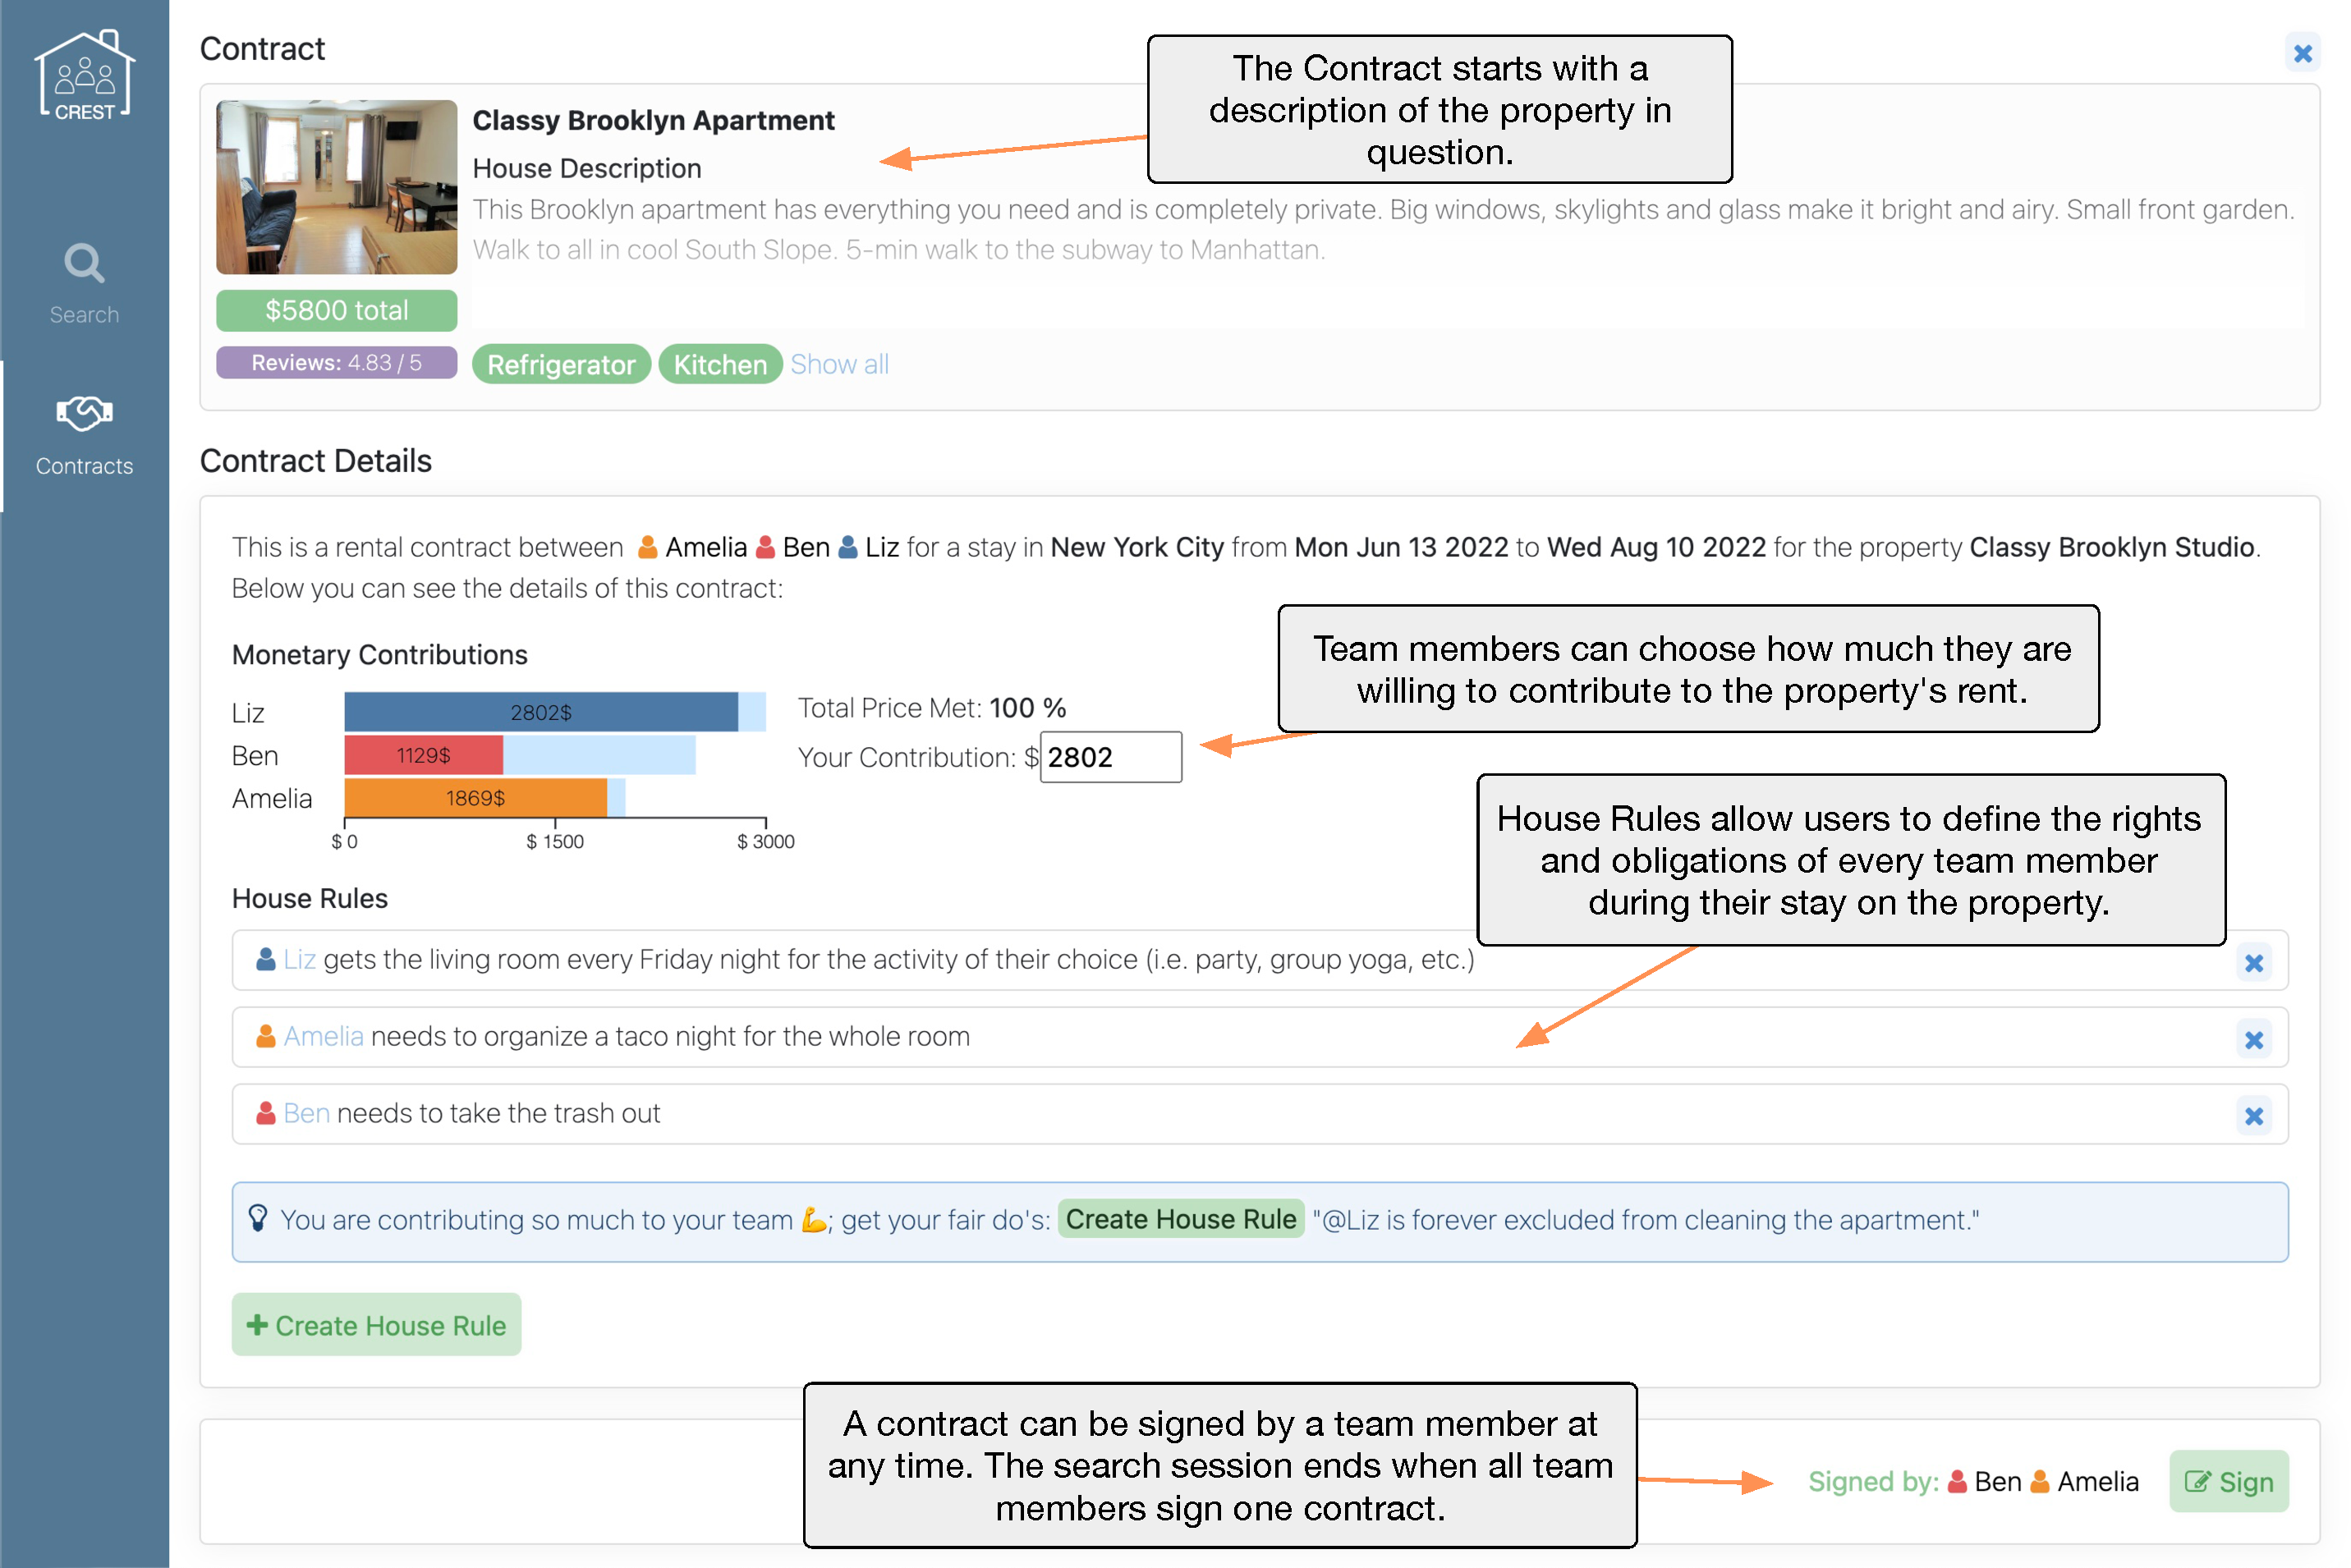
\includegraphics[width=1\textwidth]{images/ui-contracts.pdf}
    \caption{The contract page (the chat panel and \collaboRatio are cropped) shows (i) details of the property in the top panel, (ii) a visualization of monetary contributions with respect to individual budgets, (iii) a set of house rules and (iii) the users who have signed the contract so far. \cbot notifications appear where applicable to nudge the user to sign the contract if agreeable, to add house rules that lead to a more desirable agreement, or at times to consider alternative, similar properties.}
    \label{fig:ui_contracts}
\end{figure*}

\begin{figure}
    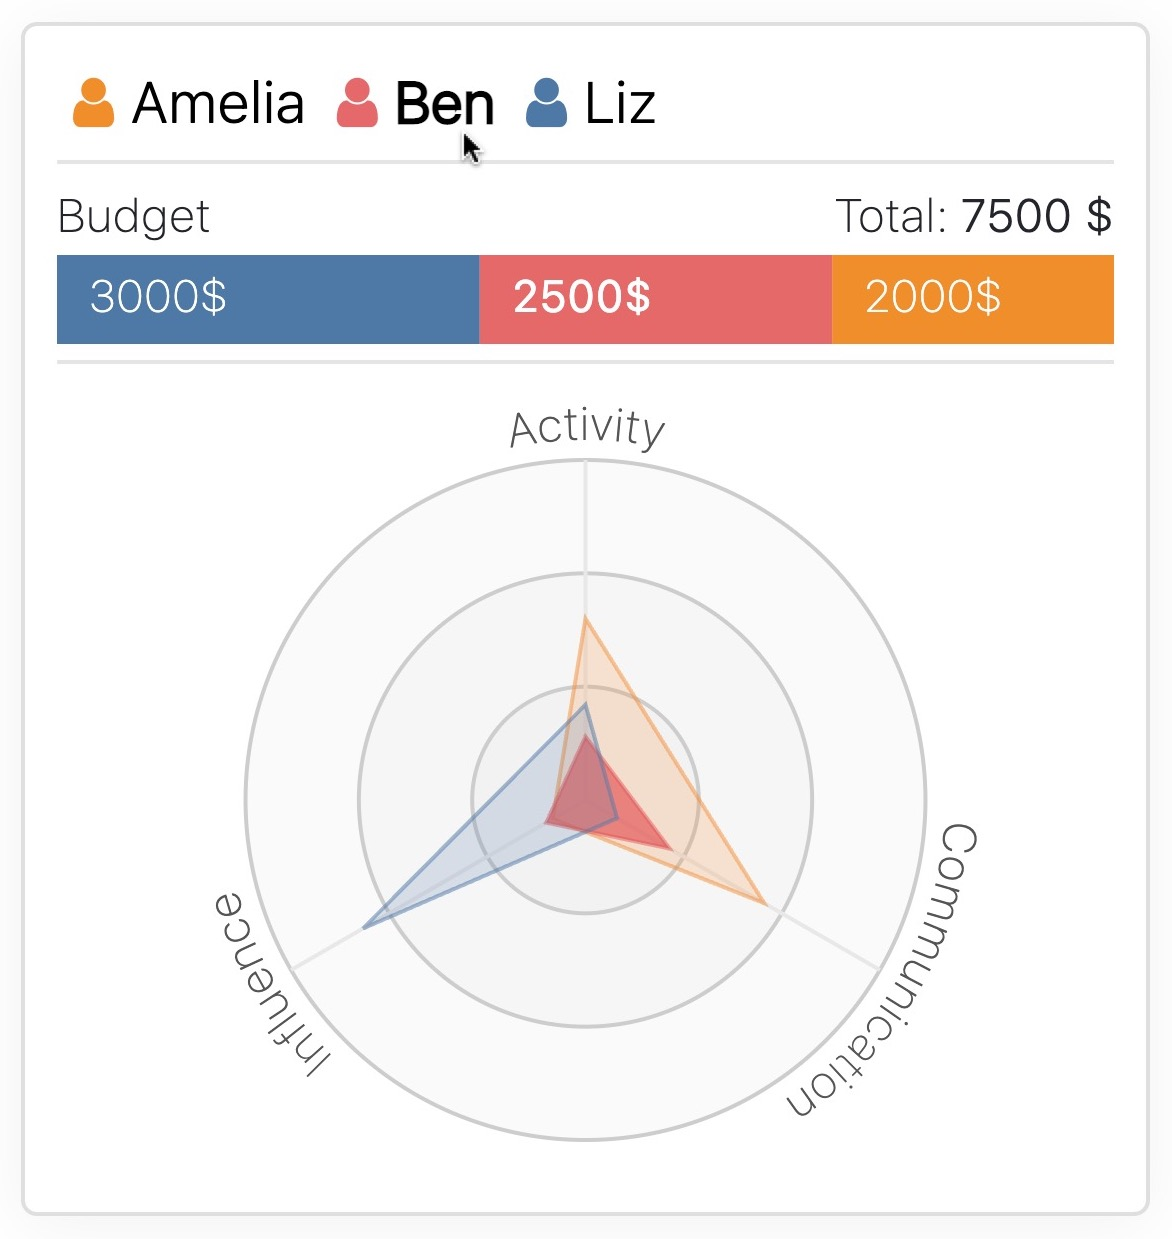
\includegraphics[width=0.45\textwidth]{images/ui-collaboratio.jpg}
    \caption{\collaboRatio provides users with a comprehensive view of their activity, communication, and influence metrics. Hovering the mouse over a username (e.g. Ben) highlights the user's collaboration patterns against the other group members' patterns.}
    \label{fig:collaboratio}
\end{figure}

To address the challenge of shifting goal posts, we carefully craft the language used in the different UI elements to create a clear understanding that the goal is to agree on a specific property. For example, each property has a \textit{"propose a contract"} button (Figure \ref{fig:ui_search}). Our intention is that this language, in comparison to \textit{"bookmark this property"} or \textit{"add to wishlist"}, will encourage users to also assess the viability of this property for the entire group before proposing it. The contract page (Figure \ref{fig:ui_contracts}) itself shifts the focus from search to a more thorough negotiation and agreement process as users examine in detail whether their collective budget is sufficient, and a house rules section prompts users to consider their co-living conditions in this specific property.

Moreover, \cbot nudges users through a variety of messages (e.g. message 1 in Table \ref{tab:messages}) to propose properties that are more appealing to them individually and the group. These messages appear within the search page and contain an action button: On clicking the button, a contract is automatically created and the user is taken to the contract page, shifting their focus from search to agreement. Messages like message 2 in Table \ref{tab:messages} highlight the benefits of a specific property and nudge users to "sign" contracts that satisfy their requirements. These examples are not exhaustive, and we envision the addition of \cbot messages in the future to accommodate new use cases. This motivated us to implement \tool with this flexibility and scalability in mind as explained in Section \ref{sssection:implementation}.



Each contract shows the number of group members that have signed the contract. Users can sign multiple contracts for all the properties they are satisfied with living in. Unsigning a contract is only allowed if the terms and conditions of the contract (e.g. allocated budgets, house rules) change. When all group members sign a contract, the group booking is finalized, an email confirmation is sent to all the group members, and the process concludes. 

Individual signatures tackle the challenge of the lack of autonomy seen in other property-booking tools. With signatures, users do not need to delegate booking to a single user that acts on the group's behalf, and they can explicitly express their agreement to a desirable contract (by signing it) or disagreement with an unsatisfactory one (by un-signing or withholding their signature from it).


\pAwareness \citeauthor{searchtogether} identify awareness as a key design principle of any collaborative search tool. Awareness is to "enable lightweight collaboration by reducing the overhead involved in explicitly asking other group members" about the task at hand. This principle addresses the discontinuity challenge. In \tool, users can easily find 
\begin{itemize}
    \item the preferences of the entire group through the \collabQueryPanel (Figure \ref{fig:ui_teams_preferences}), which appears at the top of the search page, 
    \item the degree of engagement of the group members in the collaborative task through a visualization of user activity, \collaboRatio (Figure \ref{fig:ui_search}), which appears on the side panel above the chat, 
    \item the contracts currently under consideration (the contracts page), and 
    \item for each contract who are the users who signed it, a visualization of the distribution of the users' \textit{monetary contributions}, and all its negotiated terms and conditions through the \textit{house rules} panel (Figure \ref{fig:ui_contracts}).
\end{itemize}
Since the entire state of the task is immediately accessible and persisted in the UI's components, we aid asynchronous collaboration as users do not need to wait for information-gathering rounds through chat messages or external communication channels like email. The unstructured chat medium is now better utilized for friendly conversations and more nuanced information exchange such as clarifying preference subtleties or making convincing pleas, etc. Such a free-form communication and information-exchange medium is crucial for collaborative search and agreement tasks~\cite{searchtogether, spliddit, resultsspace}. 

We will describe each component listed above, clarifying the information they provide to users.

\paragraph{\collabQueryPanel} This panel contains all team members' preferences, updated in real-time after each modification, addition, or deletion of a preference. These preferences are used to query the properties database and they influence the properties' relevance ranking in the search result. Each group member is associated with a unique and easily identifiable avatar icon and color. The \collabQueryPanel places each user's icon alongside each preference the user liked or disliked, as shown in Figure \ref{fig:ui_teams_preferences}. This collaborative query design was influenced by existing tools like \citeauthor{c-dq}'s Collaborative Dynamic Queries system, where they show "that visually externalized group awareness can support a
group in making an agreeable and satisfactory decision with
reduced cost for communication", further corroborating the importance of awareness brought forth by \citeauthor{searchtogether} \cite{c-dq,searchtogether, cometogether}.
\begin{figure*}
    \centering
    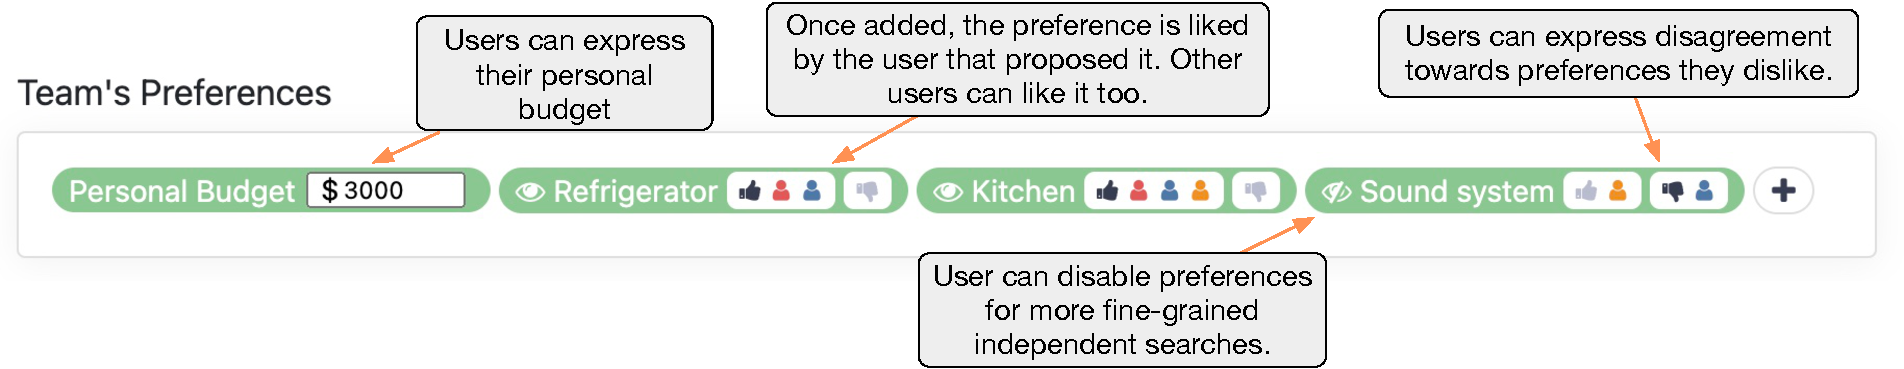
\includegraphics[width=1\textwidth]{images/ui-team-preferences.pdf}
    \caption{A screenshot of \tool's Team's Preferences panel which team members can use to conduct a collaborative query over the properties databases.}
    \label{fig:ui_teams_preferences}
\end{figure*}

Users can perform independent explorations by disabling some users' preferences. We enable this following SearchTogether's and ResultsSpace's design decision of not compromising individual search in the context of collaborative search \cite{searchtogether, resultsspace}. Instead of adding an entirely new preference, users can like or dislike preferences added by other team members. Each like to a preference increases the relevance score of the properties that satisfy it, while the inverse occurs with each dislike. \tool displays query results with the information available and needed to evaluate each property: title, location, images, price, rating, description, and the team preferences satisfied by that property. Users can sort the query results by relevance, rating, or price.

\paragraph{\collaboRatio}

To bring awareness to every team member's contribution to search and agreement, we have embedded an interactive visualization into our tool (Figure \ref{fig:collaboratio}). \collaboRatio provides visual accountability for each team member's actions. Tools like  MeetingMediator~\cite{meetingmediator} have shown that such visualizations can enhance team engagement.

\collaboRatio captures three engagement metrics: \textit{activity} or the contribution of the user to search preferences and contract proposals, \textit{influence} or the user's interaction with other users' preferences or contracts, and \textit{communication} or how often the user chats with others. These metrics are saved as simple counter variables for each user in a table in our database and are increased anytime the user meets any of the aforementioned conditions. For each user, a radial line graph connects the three metrics to form a triangle shaded with the user's assigned color. In an ideal group, the interaction dynamics would result in roughly equally-sized triangles indicating that all the group members participate equally along these three dimensions. 

\paragraph{Monetary Contributions}
Within each contract, a visualization of monetary contributions illustrates how the rent will be split among the group members (Figure \ref{fig:ui_contracts}). Each member's initial budget is also shown: this helps users get a sense of how much more or less than their initial budgets the group members are willing to contribute to meet the property's price or to settle on it.


\paragraph{House Rules}
House Rules are analogous to the clauses of a contract, defining the rights and obligations of every team member. They are unique to every property contract and are clearly presented in a house rules panel within the contract page (Figure \ref{fig:ui_contracts}). Users can write their own rules, or construct ones from several house rule templates that \tool provides (See Table \ref{tab:rules} for examples). 

\begin{table*}[]
\resizebox{0.75\linewidth}{!}{
\begin{tabular}{@{}ll@{}}
\toprule
\textbf{Template} & \textbf{Example}                                  \\ \midrule
Resource Assignment 
& {\sf \textit{userA} gets {[}the sofa | the master bedroom | the ensuite | the biggest room{]} }  \\
Resource Sharing    & 
{\sf \textit{userA} shares {[}the bedroom | the closet | the bathroom{]} with \textit{userB}, \textit{userC}, ... }\\
Chore             & 
{\sf \textit{userA} will {[}take the trash out | clean the apartment | cook lunch{]} }\\
Event Planning    & 
{\sf \textit{userA} will organize {[}a taco night | movie night{]} }                   \\
Scheduling          & 
{\sf The quiet hours are from 10:00 pm to 9:00 am | No guests on weekdays}         \\ \bottomrule
\end{tabular}
}
\vspace{0.2cm}
\caption{House Rule Templates}
\label{tab:rules}
\end{table*}


\pMediation Unlike arbitration, where an appointed judge settles conflicts or disputes within a group, mediation empowers group members to themselves resolve their conflicts with the aid of a neutral mediator. The mediator assists group members with problem-solving, negotiation and improved communication. Arbitration, including its algorithmic forms, can leave the conflicting parties feeling that the resolution was unfair, especially if it differs from their desired outcome; discussion and mediation are perceived as fairer ~\cite{algorithmicmediation}, and group relationships after mediated disputes are more likely to remain intact when compared to arbitrated ones \cite{disputeresolutionexplanation2}. Thus, we opt for mediation as a guiding design principle to address the conflicts and stalemates challenge.

\cbot acts as an impartial \textit{mediator} through chat messages, and contract or property notifications. \citeauthor{themediationprocess} describes eight roles of an ideal mediator~\cite{themediationprocess}. Influenced by \citeauthor{themediationprocess}'s work on practical mediation strategies for conflict resolution, we describe each of the ideal mediator's eight roles (quoting and summarizing from \cite{themediationprocess}) and we illustrate how the messages and notifications sent by \cbot exemplify these roles in Table \ref{tab:messages}. 


\begin{table*}[h]
\resizebox{0.85\textwidth}{!}{%
\begin{tabular}{@{}clcl@{}}
\toprule
  \multicolumn{2}{l}{\textbf{Example Message or Notification}} &
  \multicolumn{2}{l}{\textbf{Mediator Role}} \\ \midrule
1\label{msg:highestrated} &
\begin{tabular}[t]{@{}l@{}}
{\sf This property is in the top 1\% of highest-rated }\\
{\sf properties available!} \button{propose a contract}.
\end{tabular} &

\begin{tabular}[t]{@{}c@{}}
Resource Expander \\
Leader
\end{tabular} &

\begin{tabular}[t]{@{}l@{}}
Encourages users to propose a contract for a \\
property that is likely to satisfy the group.
\end{tabular}
\\[3em]

2\label{msg:satisfy_most_preferences} &
\begin{tabular}[t]{@{}l@{}}
{\sf This property satisfies most of your }\\
{\sf preferences!} \button{sign the contract}.
\end{tabular} &

\begin{tabular}[t]{@{}c@{}}
Leader
\end{tabular} &

\begin{tabular}[t]{@{}l@{}}
Moves agreement forward by getting users \\ 
to recognize the benefits of a contract \\
under consideration.
\end{tabular}
\\[3em]

3\label{msg:most_active} &
\begin{tabular}[t]{@{}l@{}}
{\sf You are your team's most active team member!}\\
{\sf Why don't you ask \textit{leastActiveUser} what} \\
{\sf they want?} \button{post a message}.
\end{tabular} &

\begin{tabular}[t]{@{}c@{}}
Comm. Opener \\
Legitimizer
\end{tabular} &

\begin{tabular}[t]{@{}l@{}}
Encourages more communication and \\
participation among group members.
\end{tabular} 

\\[3em]


4\label{msg:least_active} &
\begin{tabular}[t]{@{}l@{}}
{\sf You are your team's least active team member!}\\
{\sf Why don't you share what you would like} \\
{\sf with the group?} \button{post a message}.
\end{tabular} &

\begin{tabular}[t]{@{}c@{}}
Comm. Opener
\end{tabular} &

\begin{tabular}[t]{@{}l@{}}
Encourages more communication and \\
participation among group members.
\end{tabular} 
\\[3em]


5\label{msg:most_contrib} &
\begin{tabular}[t]{@{}l@{}}
{\sf You are contributing so much  \$\$ to your team; }\\
{\sf get your fair do's: }\\
\button{create a house rule} {\sf e.g \textit{"I get the ensuite"}}
\end{tabular} &

\begin{tabular}[t]{@{}c@{}}
Facilitator \\
Trainer
\end{tabular} &

\begin{tabular}[t]{@{}l@{}}
Promotes fair agreements through trading \\ 
and negotating monetary and non-monetary \\
contributions.
\end{tabular} 
\\[3em]

6\label{msg:least_contrib} &
\begin{tabular}[t]{@{}l@{}}
{\sf It is ok if you are paying the least, }\\
{\sf but you can }\button{create house rule} \\
{\sf of something else you can offer to} \\
{\sf sweeten the deal}
\end{tabular} &

\begin{tabular}[t]{@{}c@{}}
Facilitator \\
Trainer
\end{tabular} &

\begin{tabular}[t]{@{}l@{}}
Promotes fair agreements through trading \\
and negotating monetary and non-monetary \\
contributions.
\end{tabular} 

\\[4em]

7\label{msg:not_enough_contrib} &
\begin{tabular}[t]{@{}l@{}}
{\sf Not enough contributions to pay for this} \\
{property:} \button{reallocate contributions}
\end{tabular} &

\begin{tabular}[t]{@{}c@{}}
Agent of reality
\end{tabular} &

\begin{tabular}[t]{@{}l@{}}
Helps users construct implementable \\
contracts.
\end{tabular} 

\\[3em]

8\label{msg:pref_not_satisfied_house_rule} &
\begin{tabular}[t]{@{}l@{}}
{\sf This contract doesn't satisfy your preference}\\
{\sf for sound-proofing. Properties that do are 80\%}\\
{\sf more expensive} \button{create a house rule} to\\
{\sf negotiate a workaround or} \button{sign the contract}.
\end{tabular} &

\begin{tabular}[t]{@{}c@{}}
Agent of Reality \\
Problem Explorer
\end{tabular} &

\begin{tabular}[t]{@{}l@{}}
Challenges users with preferences that are \\
difficult to satisfy.
\end{tabular} 
\\[4em]

9\label{msg:pref_not_satisfied_alternatives} &
\begin{tabular}[t]{@{}l@{}}
{\sf This contract doesn't satisfy \textit{unsatisfiedUser}'s } \\
{\sf preference for a refrigrator. Here is a} \\
{\sf similar property that does.} \button{see property} \\
\end{tabular} &

\begin{tabular}[t]{@{}c@{}}
Legitimizer \\ 
Problem Explorer \\
Resource Expander
\end{tabular} &

\begin{tabular}[t]{@{}l@{}}
Provides similar alternatives to expand \\
settlement options
\end{tabular}

\\[3em]


10\label{msg:email}
&
\begin{tabular}[t]{@{}l@{}}
{\sf Hello there! This is a reminder that you are }\\
{\sf currently part of a group booking endeavor. }\\
{\sf Your team activities today: ...} \\
{\sf \button{Log into \tool} and find your dream property.}
\end{tabular} &

\begin{tabular}[t]{@{}c@{}}
Leader
\end{tabular} &

\begin{tabular}[t]{@{}l@{}}
This daily email reminder encourages \\
users to stay on track.
\end{tabular}
\\[3em]
   \\ \bottomrule
\end{tabular}%
}
\vspace{0.2cm}
\caption{A sample of \cbot's messages and notifications. Each message has an action button that aims to move the group booking process forward and helps users reach agreements. We associate each message with the mediator role it serves and explain how it satisfies the role.}
\label{tab:messages}
\end{table*}

\begin{enumerate}
    \item \textit{Opener of communication channels}: initiates or facilitates better communication within the group. 


    \item \textit{Legitimizer}: helps group members recognize the right of others to be involved in negotiations.

    
    \item \textit{Facilitator}: provides a procedure or forum for negotiation.

    
\item \textit{Trainer}: educates novice, unskilled, or unprepared negotiators.


\item \textit{Resource Expander}: offers resources to the group to enlarge the space of acceptable settlement options.

    
\item \textit{Problem Explorer}: enables group members to examine a conflict from different viewpoints, and assists in defining preferences or interests and looks for mutually satisfactory options.

    
\item \textit{Agent of reality}: helps build a reasonable and implementable agreement and challenges users who have extreme and unrealistic preferences.


\item \textit{Leader}: move the process forward through procedural, or on occasion, substantive—suggestions.
\end{enumerate}



All \cbot messages and notifications are displayed in a colored box and placed where most applicable in the user interface. For example, notifications that encourage users to propose a contract are placed within the property listing on the search page. Notifications that encourage users to add a house rule appear within the house-rules panel. Simple rules control the generation (and disappearance) of \cbot's messages. For example, message 3 is sent only once to the most active team member. The examples in Table \ref{tab:messages} are illustrative but not comprehensive. For example, \cbot can construct variations of message \label{msg:highestrated} to promote cheaper properties, properties that satisfy most of the team preferences, etc, as explained in Section \ref{sssection:implementation}.

\subsubsection{Implementation Specifics}
\label{sssection:implementation}

Figure \ref{fig:crest-architecture} illustrates \tool's system architecture and its main components. \tool was built using React.js, Node.js, and PostgreSQL.
Our database adheres to the data schema utilized by InsideAirbnb\cite{insideairbnb}, allowing for flexible updates of our property listings table with data from any desired city. Our React.js-based UI application enables users to access the Search Page (Figure \ref{fig:ui_search}), the Contracts Page (Figure \ref{fig:ui_contracts}), and other carefully crafted UI elements, such as \collaboRatio (Figure \ref{fig:collaboratio}), \cbot's messages (Table \ref{tab:messages}), and the Team's Preferences panel (Figure \ref{fig:ui_teams_preferences}). Our Node.js server application serves as a middleware between our UI and database. Its main components are
\collaboRatio's tracking system and \cbot's message-triggering engine.
\begin{figure}
    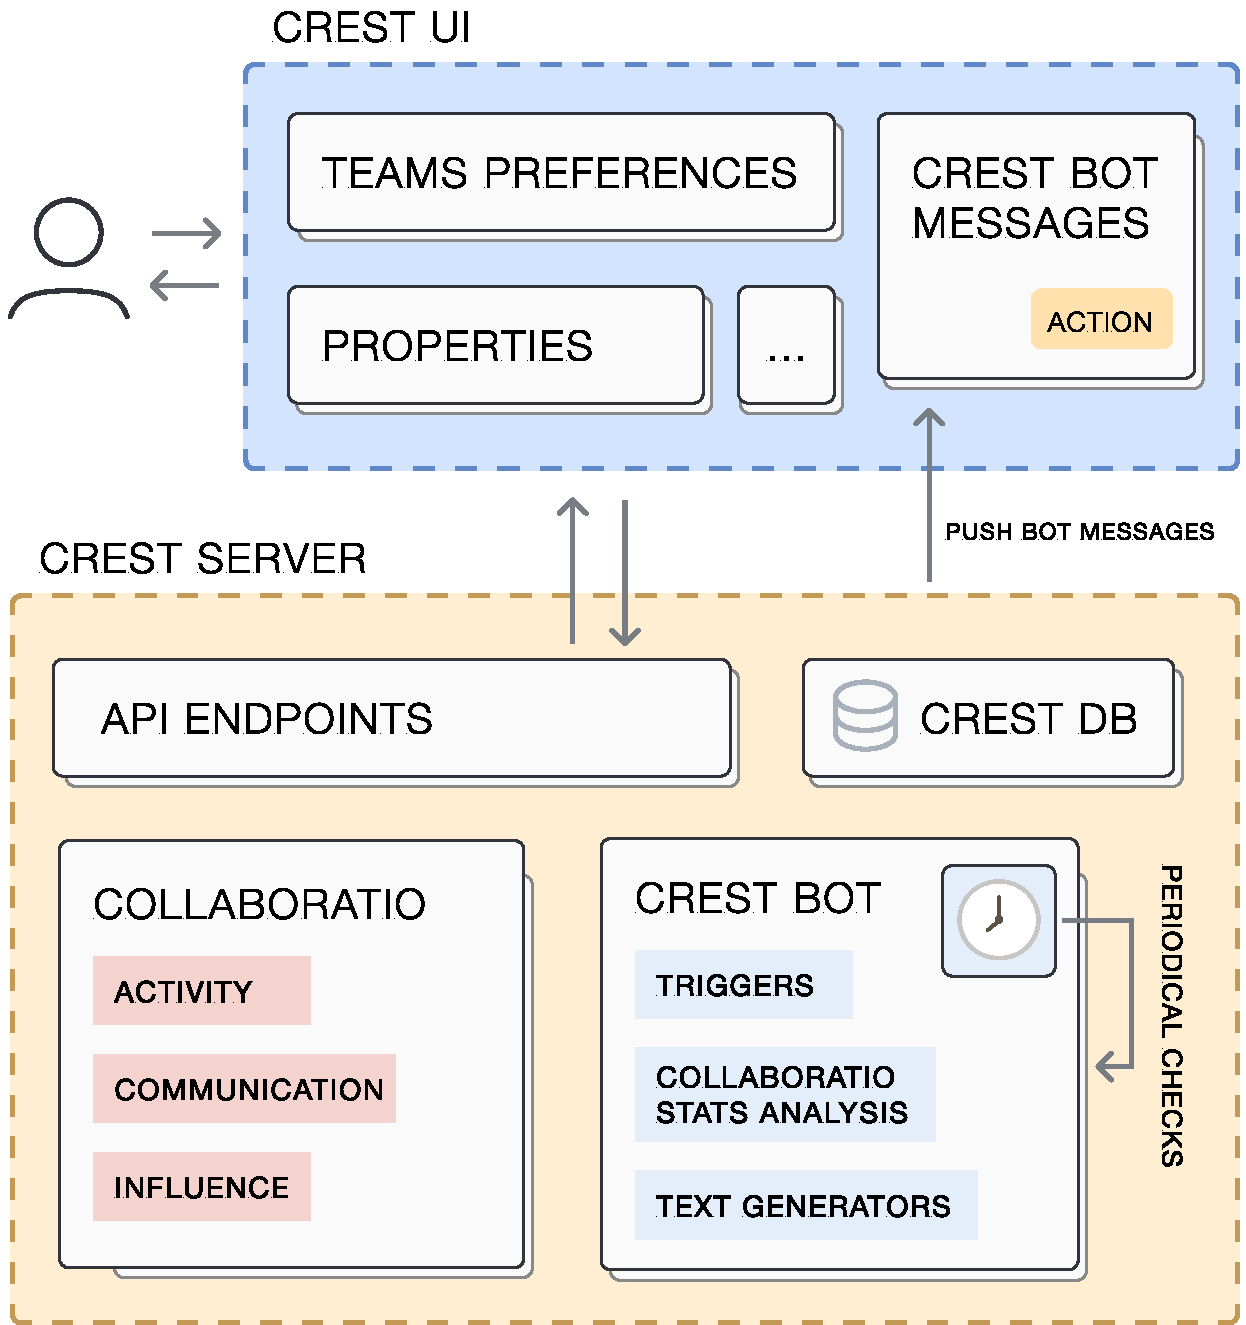
\includegraphics[width=0.55\linewidth]{images/crest-architecture.pdf}
    \caption{The system architecture of \tool.}
    \label{fig:crest-architecture}
\end{figure}


Each \cbot message is generated by a \textit{a trigger} --- an event or set of conditions that determine when the \cbot message is generated --- and an \textit{a action} --- a clickable button that meaningfully changes the state of the UI ideally towards agreement. Our \cbot message-triggering engine periodically checks for triggers, such as the addition, deletion, or modification of a preference in the Team's Preferences Panel, a change in budget contribution in a contract, or even when the system boots up, as illustrated in Figure \ref{fig:crest-architecture}. Each message's action is modeled after \pGoalCenteredFlow. Our objective is not only to notify users about significant events within \tool but also to ensure that the messages are purposeful in driving the team towards agreement through specific actions. These actions must result in a change of state in the application's UI, such as the reallocation of the team's budget to meet the contract's property price.

We have included a full list of all the triggers and their corresponding actions currently implemented in \tool in Appendix Table \ref{tab:rules-actions-table}.